\documentclass[conf]{new-aiaa}
%\documentclass[journal]{new-aiaa} % for journal papers
\usepackage[utf8]{inputenc}
\usepackage{subfig}
\usepackage{graphicx}
\usepackage{wrapfig}
\usepackage{amsmath}
\usepackage[version=4]{mhchem}
\usepackage{siunitx}
\usepackage{float}
\usepackage{algorithm}
\usepackage{algpseudocode}
\usepackage{placeins}
\usepackage{setspace}
\usepackage{amsmath}
\usepackage{longtable,tabularx}
\usepackage[colorlinks]{hyperref}% hyperlinks [must be loaded after dropping]
\hypersetup{colorlinks,breaklinks,
citecolor = blue,
urlcolor=blue,
linkcolor=blue}
\usepackage[capitalise]{cleveref}

\graphicspath{{./figs/}}

\setlength{\parindent}{0pt}
\setlength\LTleft{0pt}

\title{Oscillating Water Column (OWC) Modeling of Self-Rectifying Turbines via Parametric Performance Curves}

\author{.}


\begin{document}
%
\maketitle

\vspace{-11pt}

\section{OWC Intro}

Oscillating water column (OWC) generators simply replace the direct water to mechanical drive, or power take off (PTO), with an air-turbine interface.  \Cref{fig:example_owc} (taken from \cite{Henriques:2016aa}) shows several examples of varying designs.  

\begin{figure}[H]
\centering
\vspace{-6pt}
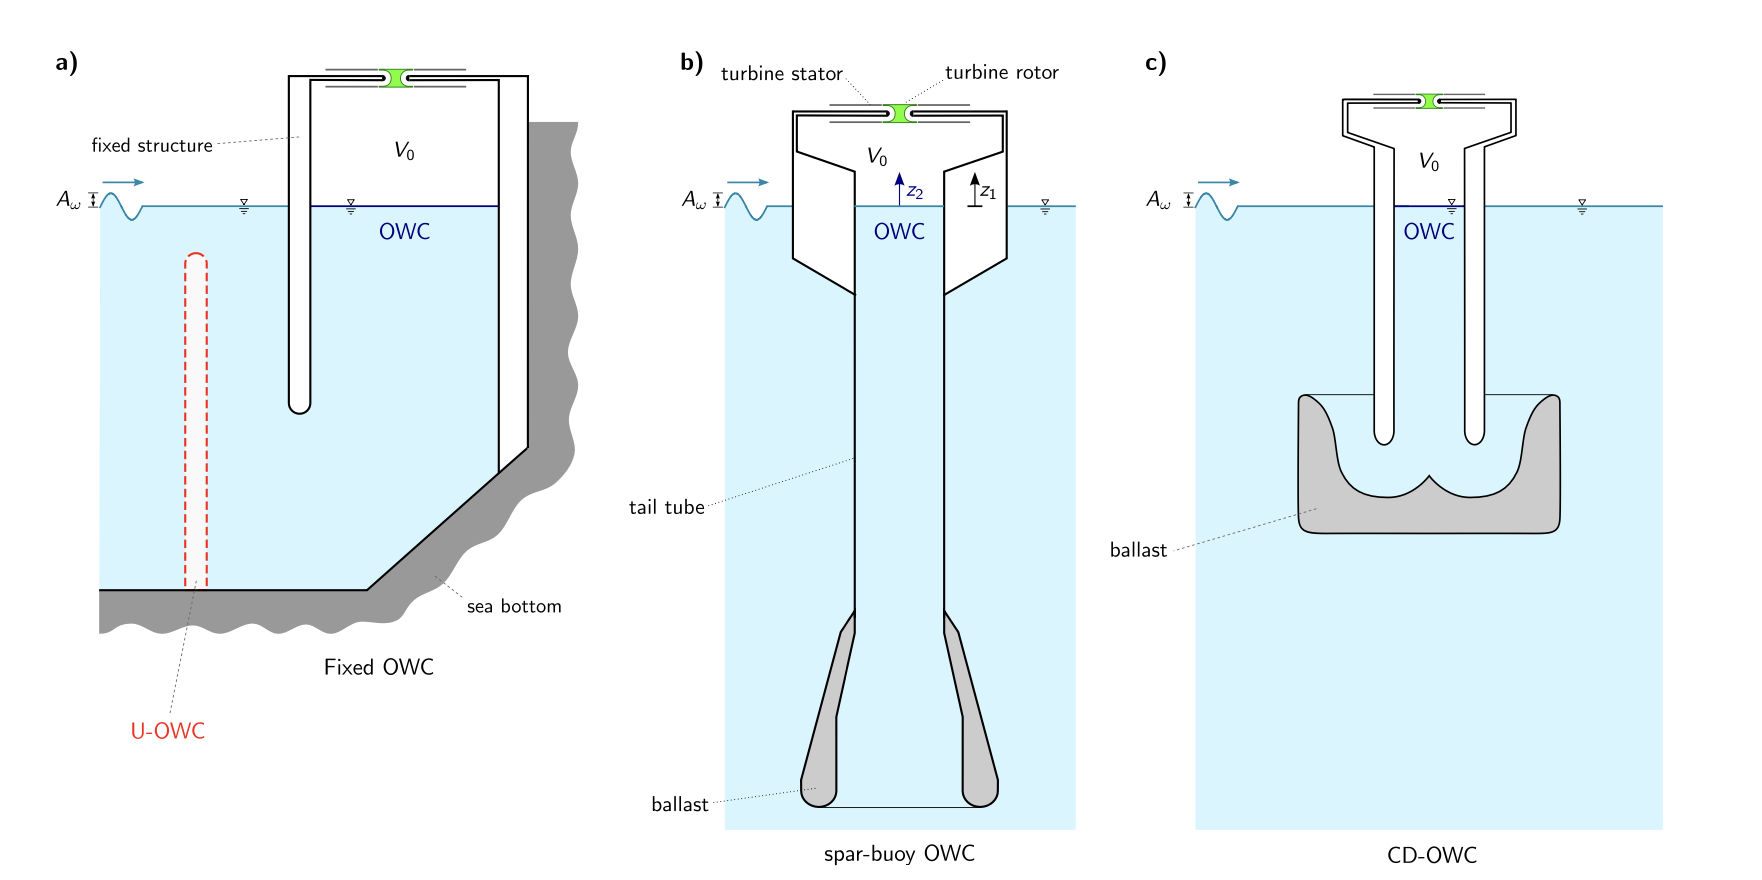
\includegraphics[trim={0cm 0cm 0cm 0cm},clip,width=0.95\textwidth]{example_owc.png}
\vspace{-6pt}
\caption{Examples of Oscillating Water Column (OWC) generators, taken from \cite{Henriques:2016aa}.}
\label{fig:example_owc}
\end{figure}

The turbines used are self-rectifying, in that they cause the turbine to spin in one direction regardless of the air flow direction.  An example of what is termed an impulse turbine is shown in \cref{fig:single_impulse_turbine} taken from \cite{Setoguchi:2004aa} and \cite{Takao:2019aa}.  There are also other designs which operate in similar ways.

\begin{figure}[H]
\centering
\vspace{-6pt}
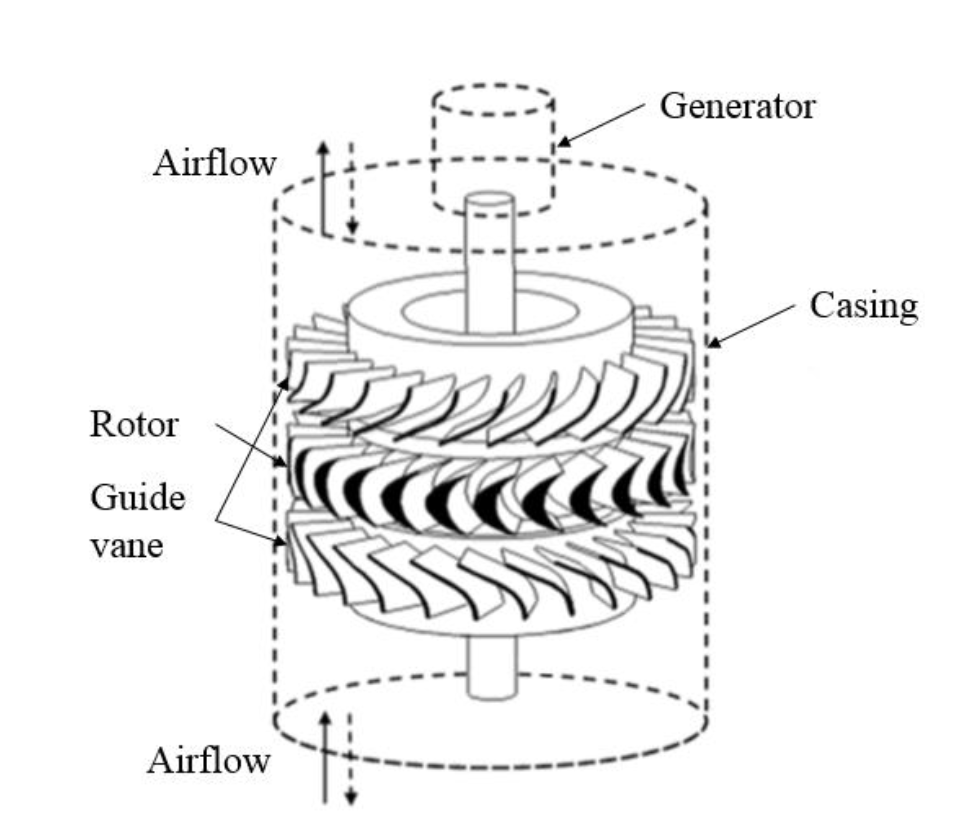
\includegraphics[trim={0cm 0cm 0cm 0cm},clip,width=0.5\textwidth]{single_impulse_turbine.png}
\vspace{-6pt}
\caption{Single rotor impulse turbine}
\label{fig:single_impulse_turbine}
\end{figure}

\section{OWC Equation Reformulation for Varying Forms of Control}

\subsection{General Equations and Normalizations for Self Rectifying Turbines}


These are the standard normalizations for self rectifying turbines taken from \cite{Setoguchi:2004aa} and \cite{Takao:2019aa}. $H_\text{blade}$ is the blade heigh (m), $c$ is chord length (m), $N_\text{blade}$ is number of blades, $R$ is the rotor outer blade radius (m)\\

Efficiency \cref{e:efficiency}

    \begin{equation}
\label{e:efficiency}
 \eta = \frac{T_0 \omega} {\Delta P Q} = \frac{C_T}{C_A \lambda_{inv}}
\end{equation}

Torque Coefficient \cref{e:CT}

    \begin{equation}
\label{e:CT}
 C_T = \frac{T_0} {\frac{1}{2}\rho(V_\text{turbine}^2 + U_R^2) H_\text{blade} c N_\text{blade} R}
\end{equation}

Input Coefficient \cref{e:CA}

    \begin{equation}
\label{e:CA}
 C_A = \frac{\Delta P_\text{turbine} Q_\text{turbine}}{\frac{1}{2}\rho(V_\text{turbine}^2 + U_R^2) H_\text{blade} c N_\text{blade} V_\text{turbine}}
\end{equation}

Inverse Tip Speed Ratio \cref{e:invTSR}

    \begin{equation}
\label{e:invTSR}
 \lambda_{inv} = \frac{V_\text{turbine}}{U_R}
\end{equation}

Blade Tip Speed \cref{e:UR}

    \begin{equation}
\label{e:UR}
U_R = \omega * R
\end{equation}

\Cref{fig:performace_curves} gives the performance curves for the turbine design in \cref{fig:single_impulse_turbine} \cite{Setoguchi:2004aa}.

\begin{figure}[H]
\centering
\vspace{-6pt}
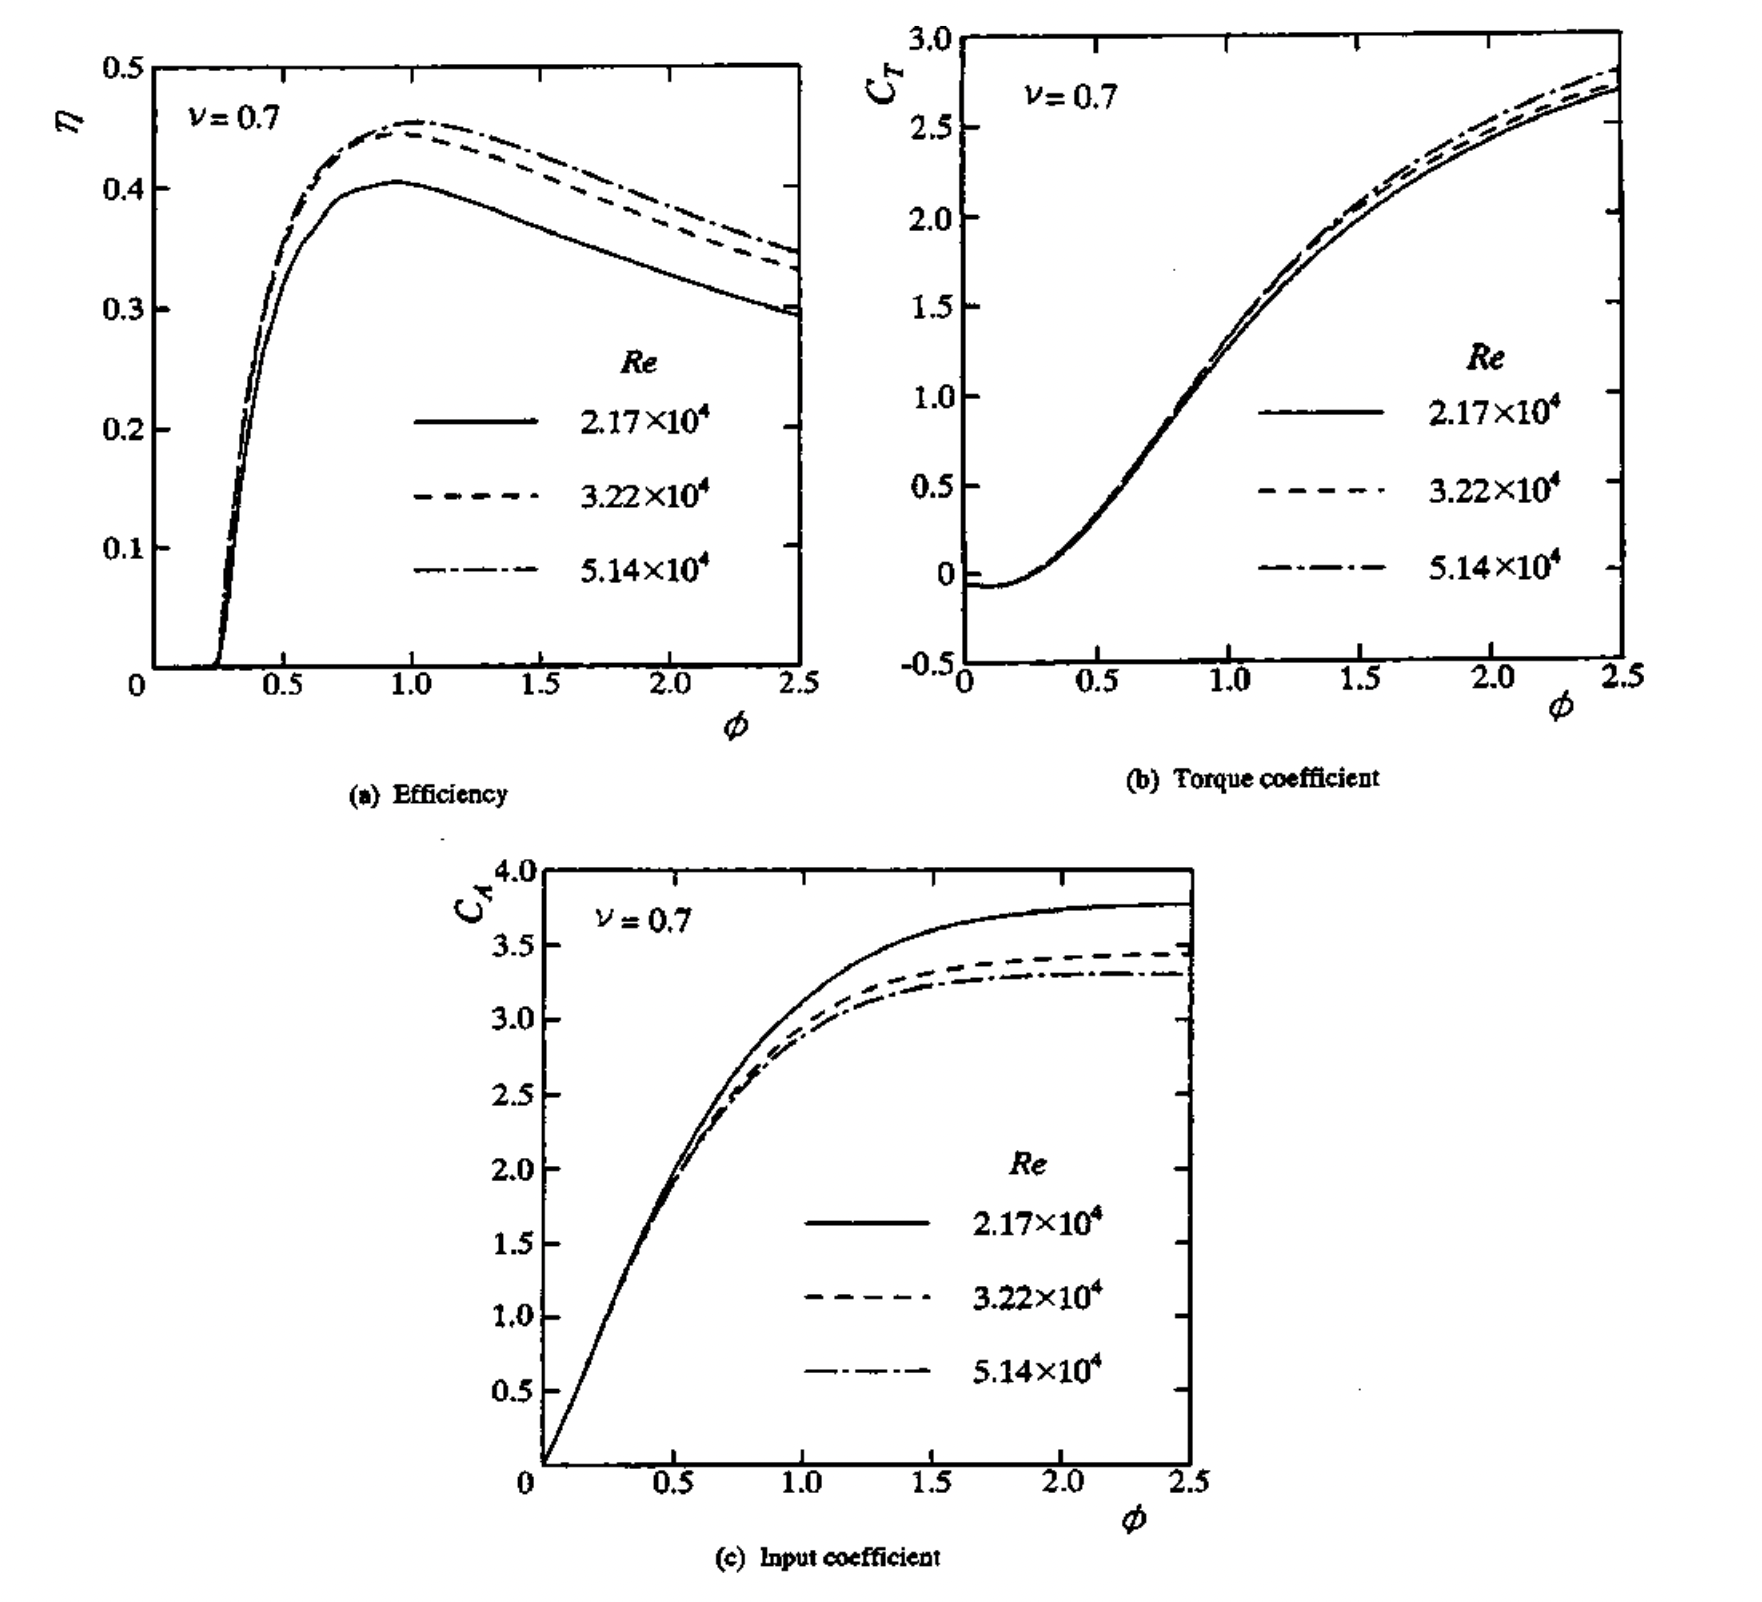
\includegraphics[trim={0cm 0cm 0cm 0cm},clip,width=0.7\textwidth]{performace_curves.png}
\vspace{-6pt}
\caption{Performance Curves}
\label{fig:performace_curves}
\end{figure}

Now, with the general equations defined, we will look at 1) adiabatic compressibility 2) A simple orifice model, 3) Omega Control, and 4) Torque Control.

\subsection{Adiabatic Compression}

Let's start by defining the various sections: 

\begin{figure}[H]
\centering
\vspace{-6pt}
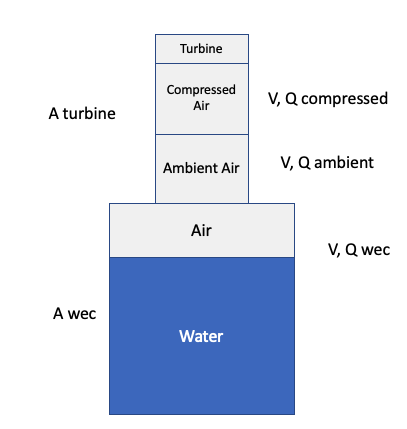
\includegraphics[trim={0cm 0cm 0cm 0cm},clip,width=0.35\textwidth]{CompressionStages.png}
\vspace{-6pt}
\caption{Sectional Diagram of the OWC}
\label{fig:CompressionStages}
\end{figure}

\Cref{e:compression} gives the standard form for adiabatic compression, or compression done without a change in entropy.  The ${\gamma}$ term, or specific heat ratio is 1.401 for air in the temperature range this turbine will be operating at. $P_\text{ambient}$ is the ambient pressure, $P_\text{turbine}$ is the compressed pressure at the turbine, $v_\text{ambient}$ is the initial volume, and $v_\text{turbine}$ is the compressed volume at the turbine.  Flow rate is simply the volume per time, and since the time is the same for both, we can substitute each volume for the respective flow rate, or $Q$.  This also holds true for the velocity $V$ since the area in the vicinity of the turbine is unchanging for our purposes.

\begin{equation}
\label{e:compression}
\frac{P_\text{turbine}}{P_\text{ambient}} = \bigg(\frac{v_\text{ambient}}{v_\text{turbine}}\bigg)^\gamma = \bigg(\frac{Q_\text{ambient}}{Q_\text{turbine}}\bigg)^\gamma = \bigg(\frac{V_\text{ambient}}{V_\text{turbine}}\bigg)^\gamma
\end{equation}

Since everything except $Q_\text{turbine}$, or the exit flowrate going into the turbine, is known, we solve for that, shown in \cref{e:flowrate}

\begin{equation}
\label{e:flowrate}
Q_\text{turbine} = \frac{Q_\text{ambient}}{\bigg(\frac{P_\text{turbine}}{P_\text{ambient}}\bigg)^\frac{1}{\gamma}}
\end{equation}

\begin{equation}
\label{e:Pcompressed}
P_\text{turbine} = \Delta P_\text{turbine} + P_\text{ambient} = \bigg(\frac{F_\text{tubine}} {A_\text{tubine}}\bigg) + P_\text{ambient} 
\end{equation}


Flow rate is constant until compression.

\begin{equation}
\label{e:Qambient}
Q_\text{ambient} = Q_\text{WEC}
\end{equation}

To round out the equations, we define the air flow rate of the WEC \cref{e:QWEC}, and the relationship between pressure and force \cref{e:Fturb}.

\begin{equation}
\label{e:QWEC}
Q_\text{WEC} = V_\text{WEC} A_\text{WEC}
\end{equation}

\begin{equation}
\label{e:Fturb}
\Delta P_\text{turbine} = \frac{F_\text{turbine}}{A_\text{turbine}}
\end{equation}

With these equations, let's reduce $Q_\text{turbine}$ \cref {e:flowrate} to known parameters, which will be useful in subsequent equations.\\


Insert \cref{e:Qambient} and \cref{e:QWEC} to reduce $Q_\text{ambient}$ and $Q_\text{WEC}$ into known parameters.
    \begin{equation}
\label{e:Qturb1}
Q_\text{turbine}  =  \frac{V_\text{WEC} A_\text{WEC} }{\bigg(\frac{P_\text{turbine}}{P_\text{ambient}}\bigg)^\frac{1}{\gamma}}
\end{equation}

Then insert \cref{e:Pcompressed} to reduce $P_\text{turbine}$ 
    \begin{equation}
\label{e:Qturb2}
Q_\text{turbine} =  \frac{V_\text{WEC} A_\text{WEC} }{\bigg(\frac{\Delta P_\text{turbine} + P_\text{ambient} }{P_\text{ambient}}\bigg)^\frac{1}{\gamma}}
\end{equation}

Simplify.
    \begin{equation}
\label{e:Qturb3}
Q_\text{turbine} =  \frac{V_\text{WEC} A_\text{WEC}} {\bigg(\frac{\Delta P_\text{turbine} }{P_\text{ambient} } + 1\bigg)^\frac{1}{\gamma}}
\end{equation}

Note that this also applies to $V_\text{turbine}$ in the following way.  Take \cref{e:flowrate} and swap for $V_\text{turbine}$
    \begin{equation}
\label{e:V_turb1}
V_\text{turbine} = \frac{V_\text{ambient}}{\bigg(\frac{P_\text{turbine}}{P_\text{ambient}}\bigg)^\frac{1}{\gamma}}
\end{equation}

$V_\text{ambient}$ is the velocity corrected for conservation of mass.
 \begin{equation}
\label{e:Vambient}
V_\text{ambient} = \frac{V_\text{WEC} A_\text{WEC}} {A_\text{turbine}}
\end{equation}

Inserting these two and simplifying gives

    \begin{equation}
\label{e:V_turb2}
V_\text{turbine} =  \frac{V_\text{WEC} A_\text{WEC}} {A_\text{turbine} \bigg(\frac{\Delta P_\text{turbine} }{P_\text{ambient} } + 1\bigg)^\frac{1}{\gamma}}
\end{equation}

Another useful equation is to get the inverse TSR into known terms by starting with \cref{e:invTSR}, inserting \cref{e:UR}, and inserting \cref{e:V_turb2}:
    \begin{equation}
\label{e:TSR2}
\lambda_{inv} =  \frac{V_\text{WEC} A_\text{WEC}} {A_\text{turbine} \bigg(\frac{\Delta P_\text{turbine} }{P_\text{ambient} } + 1\bigg)^\frac{1}{\gamma} \omega R}
\end{equation}

Reducing for incompressibility drops the terms in parenthesis.
    \begin{equation}
\label{e:TSRincompressible}
\lambda_{inv} =  \frac{V_\text{WEC} A_\text{WEC}} {A_\text{turbine} \omega R}
\end{equation}



\subsection{Simple Restricting Orifice}

WecOptTool is already built to apply a direct force on the wave energy converter (WEC).  This force, in combination with the velocity of the WEC via the dynamics gives the power taken off of the system (and other efficiency reductions can be modeled through generator losses etc).  For our purposes, we focus on the power extracted from the system.  For the direct PTO, the power is shown in \cref{e:P_PTO} and is proportional to the force exerted, and the resulting dynamic velocity.  These equations assume 100\% power conversion efficiency.

\begin{equation}
\label{e:P_PTO}
\text{Power} = F_\text{WEC} V_\text{WEC}
\end{equation}

When we start extracting power from the air, we use the following equation, where the change in pressure is due to the theoretical change in orifice restriction in conjunction with the wec dynamics, similar to the piston pushing back on the water.

\begin{equation}
\label{e:P_air}
\text{Power} = \Delta P_\text{turbine} Q_\text{turbine}
\end{equation}

But we need to recall that the force and pressure are related and we need a relation between $F_\text{WEC}$ and $F_\text{turbine}$ since the pressure is constant between the two secitons.

\begin{equation}
\label{e:F_turb1}
\frac{F_\text{turbine}}{A_\text{turbine}} = \frac{F_\text{WEC}}{A_\text{WEC}}
\end{equation}

\begin{equation}
\label{e:F_turb2}
F_\text{turbine} = \frac{F_\text{WEC} A_\text{turbine}}{A_\text{WEC}}
\end{equation}

To implement \cref{e:P_air} as a function in WecOptTool, let's combine the quations, working backwards, starting with \cref{e:P_air}, and substiting \cref{e:Qturb3} and \cref{e:Fturb} and to get \cref{e:P_sub1}

\begin{equation}
\label{e:P_sub1}
\text{Power} = \bigg( \frac{F_\text{turbine}}{A_\text{turbine}}\bigg) \Bigg(  \frac{V_\text{WEC} A_\text{WEC}} {\bigg(\frac{\frac{F_\text{turbine}}{A_\text{turbine}}}{P_\text{ambient} } + 1\bigg)^\frac{1}{\gamma}} \Bigg)
\end{equation}

We can simplify this to:

\begin{equation}
\label{e:P_sub5}
\text{Power} = \frac{F_\text{turbine} V_\text{WEC} A_\text{WEC} }{A_\text{turbine} \bigg(\frac{F_\text{tubine}} {A_\text{tubine} P_\text{ambient}} + 1 \bigg)^\frac{1}{\gamma}}
\end{equation}

And then insert \cref{e:F_turb2} to $F_\text{turbine}$ to the known $F_\text{WEC}$

\begin{equation}
\label{e:P_sub52}
\text{Power} = \frac{\frac{F_\text{WEC} A_\text{turbine}}{A_\text{WEC}} V_\text{WEC} A_\text{WEC} }{A_\text{turbine} \bigg(\frac{\frac{F_\text{WEC} A_\text{turbine}}{A_\text{WEC}}} {A_\text{tubine} P_\text{ambient}} + 1 \bigg)^\frac{1}{\gamma}}
\end{equation}

Simplify:

\begin{equation}
\label{e:P_sub7}
\text{Power} = \frac{F_\text{WEC}  V_\text{WEC} }{\bigg(\frac{F_\text{WEC}} {A_\text{WEC} P_\text{ambient}} + 1 \bigg)^\frac{1}{\gamma}}
\end{equation}

The incompressible version is as follows with everything dropping out.

\begin{equation}
\label{e:P_sub8}
\text{Power} =  F_\text{WEC} V_\text{WEC}
\end{equation}

If we retain the $\Delta P_\text{turbine}$ frame of reference, then we get the following:

\begin{equation}
\label{e:P_sub6}
\text{Power} = \frac{\Delta P_\text{turbine} V_\text{WEC} A_\text{WEC}} {\bigg(\frac{\Delta P_\text{turbine} }{P_\text{ambient} } + 1\bigg)^\frac{1}{\gamma}}
\end{equation}

If we assume incompressibility, then the bottom $\Delta P_\text{turbine}$ equals 0 and the items in parenthesis are always 1.

\begin{equation}
\label{e:P_sub6_incompressible}
\text{Power} = \Delta P_\text{turbine} V_\text{WEC} A_\text{WEC}
\end{equation}

\subsection{Omega Control}

To control via the turbine rotation rate directly, we solve \cref{e:CA} for $\Delta P_\text{turbine}$ and substitute $U_R$ with the blade tip speed $\omega R$.  Also keep in mind that $C_A$ is actually a performance curve as shown in \cref{fig:performace_curves}.

    \begin{equation}
\label{e:CA2}
C_A = f(\lambda_{inv}) = f\bigg(\frac{V_\text{turbine}}{\omega R}\bigg)
\end{equation}

    \begin{equation}
\label{e:deltaP}
\Delta P_\text{turbine} = \frac{C_A \frac{1}{2}\rho \Bigg(V_\text{turbine}^2 + \bigg(\omega R \bigg)^2 \Bigg) H_\text{blade} c N_\text{blade} V_\text{turbine}} { Q_\text{turbine}}
\end{equation}

However, we need to substitute in \cref{e:Qturb3} to reduce $Q_\text{turbine}$ into known parameters.

    \begin{equation}
\label{e:deltaP2}
\Delta P_\text{turbine} = \frac{C_A \frac{1}{2}\rho \Bigg(V_\text{turbine}^2 + \bigg(\omega R \bigg)^2 \Bigg) H_\text{blade} c N_\text{blade} V_\text{turbine}} { \frac{V_\text{WEC} A_\text{WEC}^2} {A_\text{turbine} \bigg(\frac{\Delta P_\text{turbine} }{P_\text{ambient} } + 1\bigg)^\frac{1}{\gamma}}}
\end{equation}


Simplify:
    \begin{equation}
\label{e:deltaP3}
\Delta P_\text{turbine} = \frac{C_A \frac{1}{2}\rho \Bigg(V_\text{turbine}^2 + \bigg(\omega R \bigg)^2 \Bigg) H_\text{blade} c N_\text{blade} V_\text{turbine} A_\text{turbine} \bigg(\frac{\Delta P_\text{turbine}} {P_\text{ambient}} + 1 \bigg)^\frac{1}{\gamma}} {V_\text{WEC} A_\text{WEC}^2}
\end{equation}


Now substitute in \cref{e:V_turb2} to reduce $V_\text{turbine}$ into known parameters.

    \begin{equation}
\label{e:deltaP4}
\Delta P_\text{turbine} = \frac{C_A \frac{1}{2}\rho \Bigg(\Bigg(\frac{V_\text{WEC} A_\text{WEC}} {A_\text{turbine} \bigg(\frac{\Delta P_\text{turbine} }{P_\text{ambient} } + 1\bigg)^\frac{1}{\gamma}}\Bigg)^2 + \bigg(\omega R \bigg)^2 \Bigg) H_\text{blade} c N_\text{blade} \Bigg(\frac{V_\text{WEC} A_\text{WEC}} {A_\text{turbine} \bigg(\frac{\Delta P_\text{turbine} }{P_\text{ambient} } + 1\bigg)^\frac{1}{\gamma}}\Bigg) A_\text{turbine} \bigg(\frac{\Delta P_\text{turbine}} {P_\text{ambient}} + 1 \bigg)^\frac{1}{\gamma}} {V_\text{WEC} A_\text{WEC}^2}
\end{equation}

Simplify:
    \begin{equation}
\label{e:deltaP5}
\Delta P_\text{turbine} = \frac{C_A \frac{1}{2}\rho \Bigg(\Bigg(\frac{V_\text{WEC} A_\text{WEC}} {A_\text{turbine} \bigg(\frac{\Delta P_\text{turbine} }{P_\text{ambient} } + 1\bigg)^\frac{1}{\gamma}}\Bigg)^2 + \bigg(\omega R \bigg)^2 \Bigg) H_\text{blade} c N_\text{blade} } {A_\text{WEC}}
\end{equation}

This equation requires an implicit solve due to the compressibility.  If we were to rederive the equations without compressibility, this would simply assume conservation of mass to get the change in velocity at the turbine, related to the wec velocity, and reduce as follows:

    \begin{equation}
\label{e:deltaPincomp}
\Delta P_\text{turbine} = \frac{C_A \frac{1}{2}\rho \Bigg(\Bigg(\frac{V_\text{WEC} A_\text{WEC}} {A_\text{turbine} }\Bigg)^2 + \bigg(\omega R \bigg)^2 \Bigg) H_\text{blade} c N_\text{blade} } {A_\text{WEC}}
\end{equation}

We can then insert either \cref{e:deltaP5} or \cref{e:deltaPincomp} into \cref{e:P_sub6} or \cref{e:P_sub6_incompressible} depending on if we are modeling compressibility and handling the implicit solve or not. \\

 Then to get the power coming out of the turbine, we can multiply the resulting power by the turbine efficiency, recalling that the efficiency is also a performance curve dependent on the inverse tip speed ratio (use \cref{e:TSR2} or \cref{e:TSRincompressible} depending on if you are modeling compressibility and solving the implicit equations).
 
     \begin{equation}
\label{e:CA2}
\eta = f(\lambda_{inv})
\end{equation}

\subsection{Torque Control}

To control via torque, we undergo a similar derivation process as for omega, starting with \cref{e:CT} and solving for $\omega$.  Let's take if one step at a time

    \begin{equation}
\label{e:CT1}
(V_\text{turbine}^2 + U_R^2) = \frac{T_0} { C_T \frac{1}{2}\rho H_\text{blade} c N_\text{blade} R}
\end{equation}

    \begin{equation}
\label{e:CT1}
(\omega R)^2 = \frac{T_0} { C_T \frac{1}{2}\rho H_\text{blade} c N_\text{blade} R} - V_\text{turbine}^2 
\end{equation}

    \begin{equation}
\label{e:CT1}
\omega = \frac{1}{R} \sqrt{\frac{T_0} { C_T \frac{1}{2}\rho H_\text{blade} c N_\text{blade} R} - V_\text{turbine}^2 }
\end{equation}

Let's insert $V_\text{turbine}$ from \cref{e:V_turb2}
    \begin{equation}
\label{e:CT1}
\omega = \frac{1}{R} \sqrt{\frac{T_0} { C_T \frac{1}{2}\rho H_\text{blade} c N_\text{blade} R} - \Bigg(  \frac{V_\text{WEC} A_\text{WEC}} {A_\text{turbine} \bigg(\frac{\Delta P_\text{turbine} }{P_\text{ambient} } + 1\bigg)^\frac{1}{\gamma}} \Bigg)^2 }
\end{equation}

Assuming incompressibility would give

    \begin{equation}
\label{e:CT2}
\omega = \frac{1}{R} \sqrt{\frac{T_0} { C_T \frac{1}{2}\rho H_\text{blade} c N_\text{blade} R} - \Bigg(  \frac{V_\text{WEC} A_\text{WEC}} {A_\text{turbine} } \Bigg)^2 }
\end{equation}

\Cref{e:CT1} is then inserted into \cref{e:deltaP5}, which is then inserted into \cref{e:P_sub6}, and multiplied by the resulting efficiency from the resulting inverse tip speed ratio \cref{e:TSR2}, and likewise for the incompressible versions. However, even for the incompressible version, since $C_T$ is dependent on $\omega$, it requires an implicit solve.  

\section{Implementation}

Let's start with the wavebot tutorial, with the following flowchart \cref{fig:WecOptFlowOrig}.

\begin{figure}[H]
\centering
\vspace{-6pt}
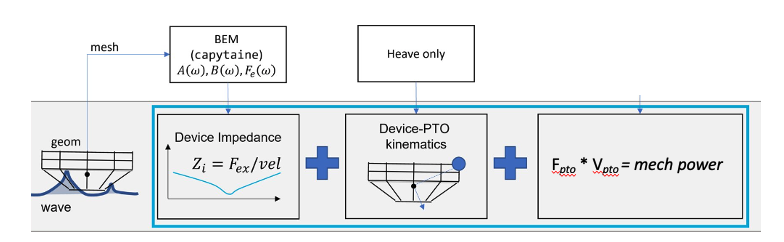
\includegraphics[trim={0.2cm 0cm 0cm 0cm},clip,width=0.9\textwidth]{WEC_mechanicalPower.png}
\vspace{-6pt}
\caption{Performance Curves}
\label{fig:WecOptFlowOrig}
\end{figure}

When solved with WecOptTool, we get and optimal mechanical average power of -101.15W.

\begin{figure}[H]
\centering
\vspace{-6pt}
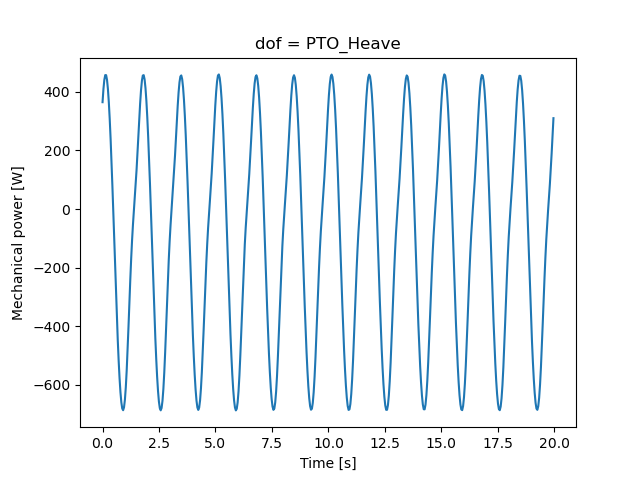
\includegraphics[trim={0.0cm 0cm 0cm 0cm},clip,width=0.6\textwidth]{PTO_1.png}
\vspace{-6pt}
\caption{Performance Curves}
\label{fig:WecOptFlowOrig}
\end{figure}

\subsection{Restricting Orifice}

Since we showed earlier that the incompressible version of the simple restricting orifice gives the same solution as the direct PTO, we use the compressible version \cref{e:P_sub7} in lieu of the direct FxV to get the mechanical average power.  

If we assume a wec area of 1 m2, the resulting pressure is nearly insignificant compared to the ambient pressure and the solution is nearly identical in control form and average power (-101.19W).  If we change the wec area to 0.1 m2, then compressibility starts to play a factor, and we can get a slight increase in total power as the controller is able to use the air column as a spring, resulting in a mechanical average power of -105.43 W. This assumes that the force can be negative, or in other words, energy can be put into the system to decompress the air, which is physically possible for a self rectifying turbine, up to the point that the airflow is reversed from the direction of motion.

\begin{figure}[H]
\centering
\vspace{-6pt}
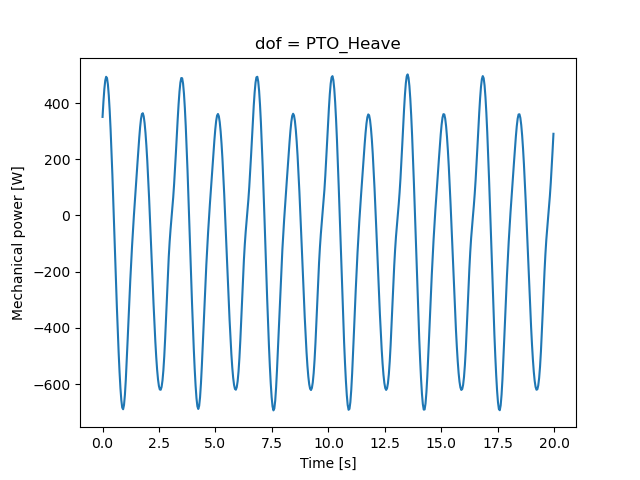
\includegraphics[trim={0.0cm 0cm 0cm 0cm},clip,width=0.6\textwidth]{choke_1.png}
\vspace{-6pt}
\caption{Performance Curves}
\label{fig:choke_1}
\end{figure}

To give a relative understanding of the compression, recall that 1 atm is 101325.0 pa, which is $P_\text{ambient}$.  If the force is 2000 N (the constraint in the PTO example) and the area is 0.1 m2 then the pressure is 20,000 pa, or about 20\% of the ambient pressure, while if the area is 1.0 m2, then it is only 2\% of the ambient pressure.

\subsection{Incompressible Omega Control}

Now to incorporate the performance curves from the self rectifying turbine.  Let's start with the incompressible version of the omega control equations to bypass the implicit solve for now.  The only other implementation detail is that we will need to provide the force on the WEC since it is now no longer a design variable, but a calculated value from the omega control.  We also need to create splines for the Ca and efficiency curves. However, it becomes difficult with getting everything scaled and started so that the solver will solve...

\subsection{Compressible Omega Control}

Because this requires an implicit solve (compressibility requires the knowledge of the change in pressure, for which we are solving for), we must either run a 1D root finder within WecOptTool, or run the root finder outside and create a 2D lookup spline.  Alternatively, we can add more state variables to the $X_opt$ array and use the optimizer to drive the residual to zero.

\subsection{Incompressible Torque Control}

Incompressible torque control also this requires an implicit solve (calculating omega from torque requires the torque coefficient, which is dependent on knowing omega), so it requires the same process.

\subsection{Compressible Torque Control}

When we include compressibility with the torque control, this reintroduces the issue with the change in pressure, and so we must use a 2D root finder and preprocess, or alternatively, we can add more state variables to the $X_opt$ array and use the optimizer to drive both residuals to zero.

%\cite{Shanghavi:2012aa} 2012Shanghavi\_TurbineShadingPV\_SurfacePlots\_Stay4Daway


\bibliography{sources_bibtex}

\end{document}
